\appendix
\chapter{Bilder}
\section{Creditkauf auf Fotor}

\begin{figure}[H]
\centering
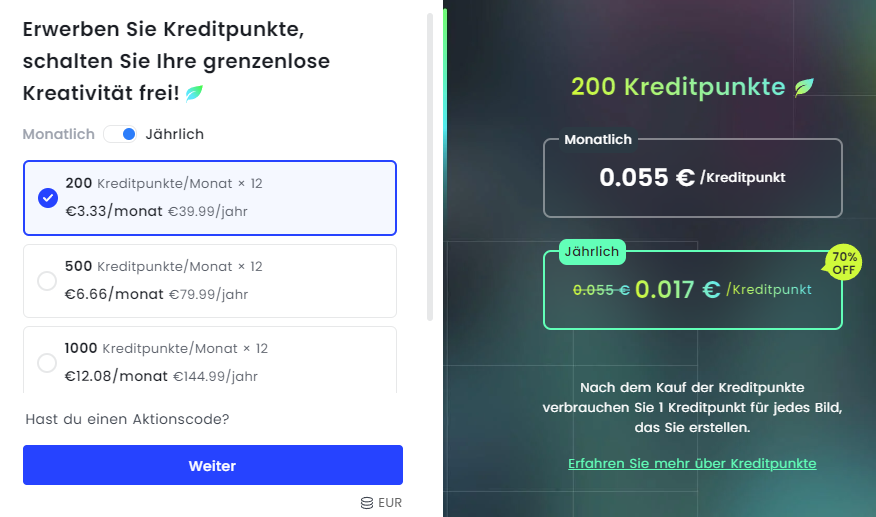
\includegraphics[width=1\linewidth]{Images/Creditkauf auf Fotor.png}\\
\caption{Pop-up Fenster von Fotor.com für den Creditkauf}
\label{fig:Fotor_Credits}
\end{figure}

\section{Reforge LaTeX-Ausgabetest}

\begin{figure}[H]
\centering
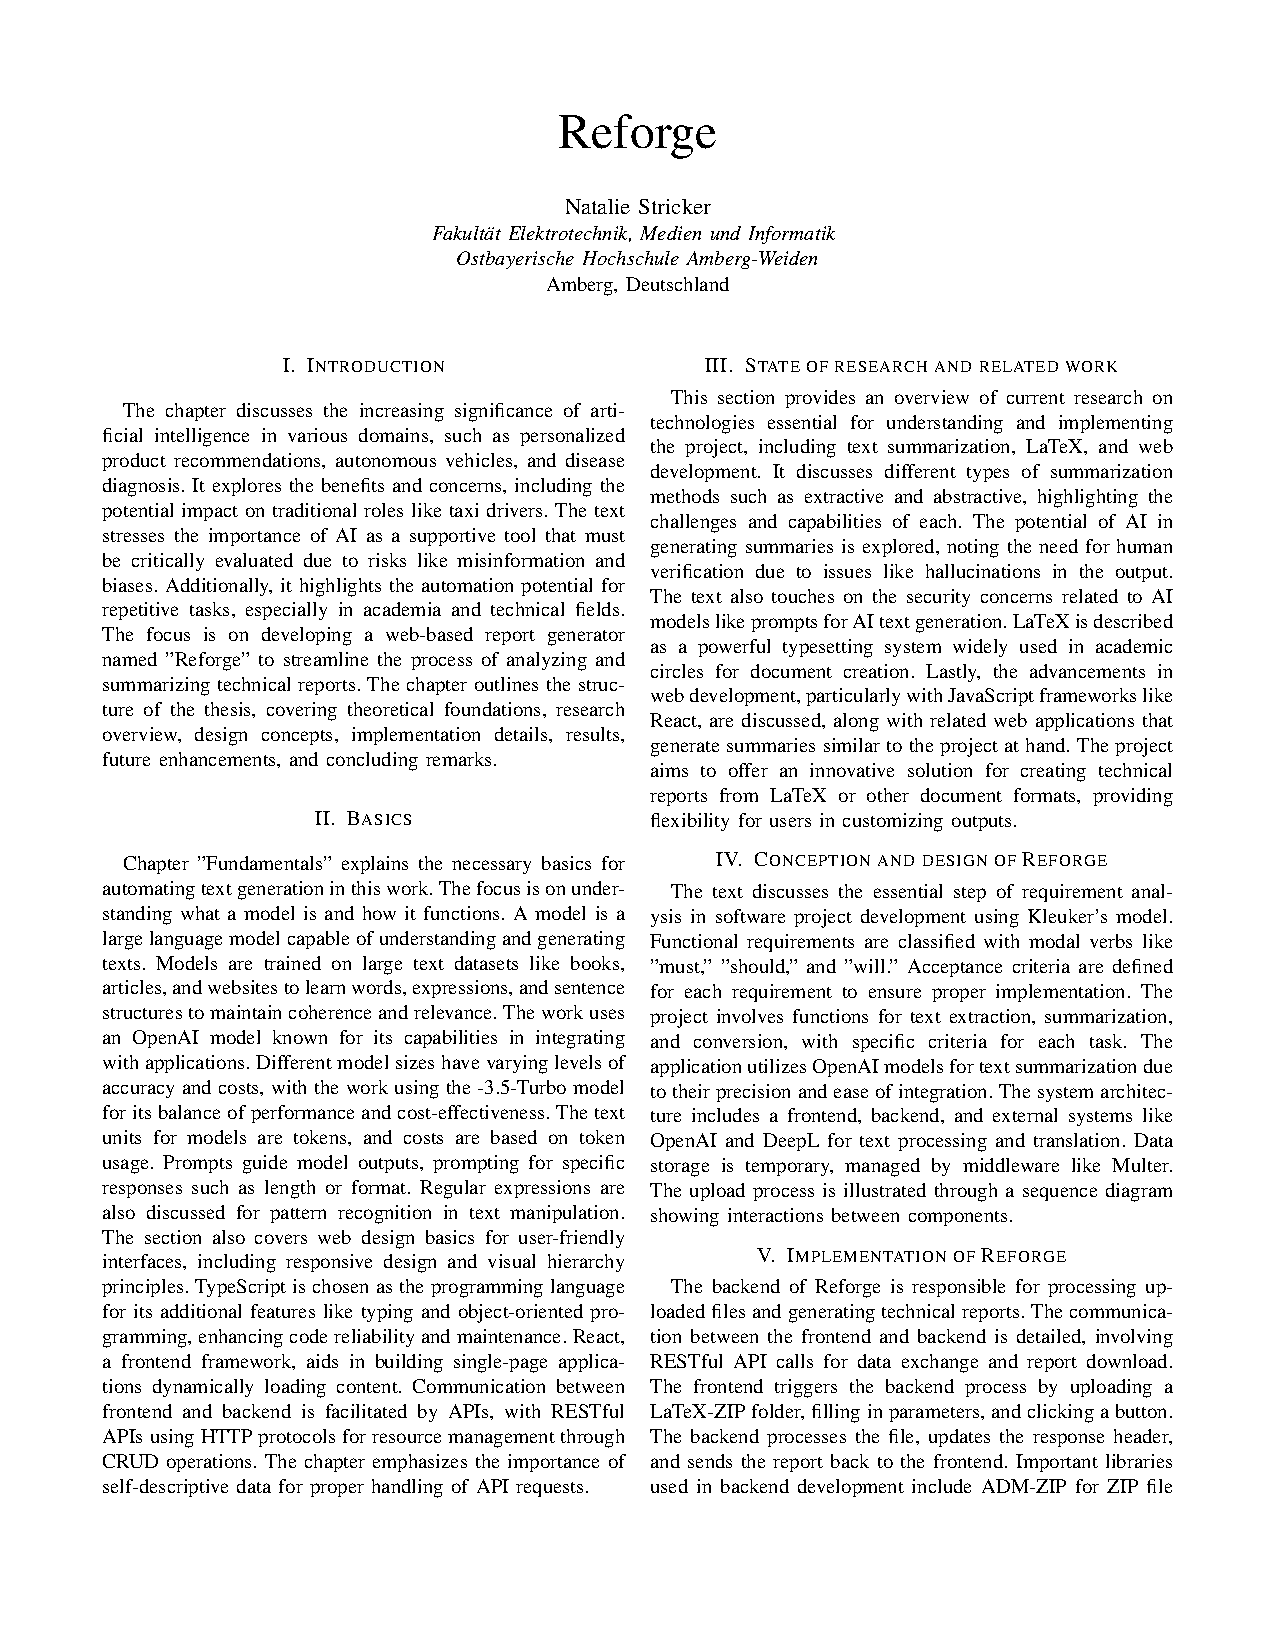
\includegraphics[width=1\linewidth]{Images/ReforgeTestGen1.pdf}\\
\caption{Reforge LaTeX-Ausgabetest auf Basis dieser Bachelorarbeit, Seite eins}
\label{fig:Reforge_testgen1}
\end{figure}

\begin{figure}[H]
\centering
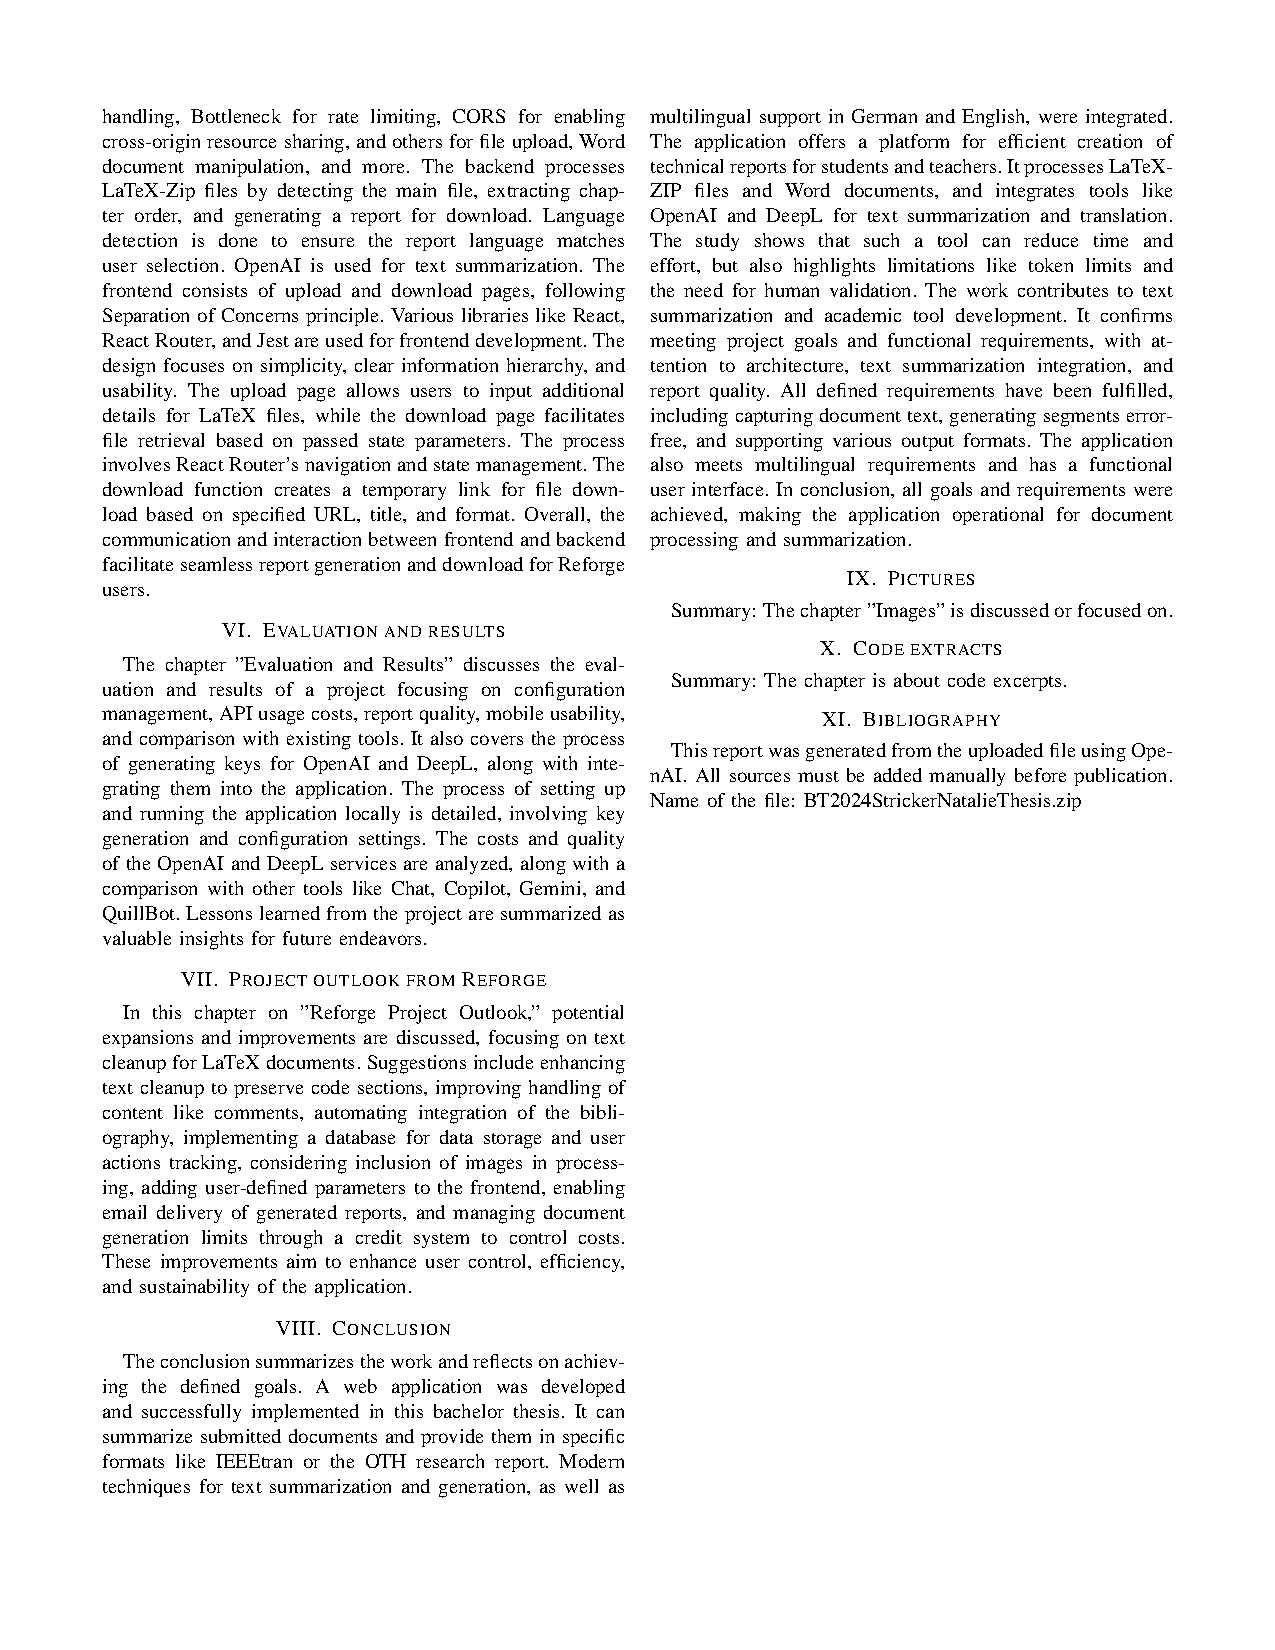
\includegraphics[width=1\linewidth]{Images/ReforgeTestGen2.pdf}\\
\caption{Reforge LaTeX-Ausgabetest auf Basis dieser Bachelorarbeit, Seite zwei}
\label{fig:Reforge_testgen2}
\end{figure}

\section{Reforge DOCX-Ausgabetest}

\begin{figure}[H]
\centering

\includegraphics[width=0.9\linewidth]{Images/ReforgeDOCXGen1.pdf}\\
\caption{Reforge \ac{DOCX}-Ausgabetest auf Basis dieser Bachelorarbeit, Seite eins}
\label{fig:ReforgeDOCXGen1}
\end{figure}

\begin{figure}[H]
\centering

\includegraphics[width=0.9\linewidth]{Images/ReforgeDOCXGen2.pdf}\\
\caption{Reforge \ac{DOCX}-Ausgabetest auf Basis dieser Bachelorarbeit, Seite zwei}
\label{fig:ReforgeDOCXGen2}
\end{figure}

\section{ChatGPT Test 2}

\begin{figure}[H]
\centering
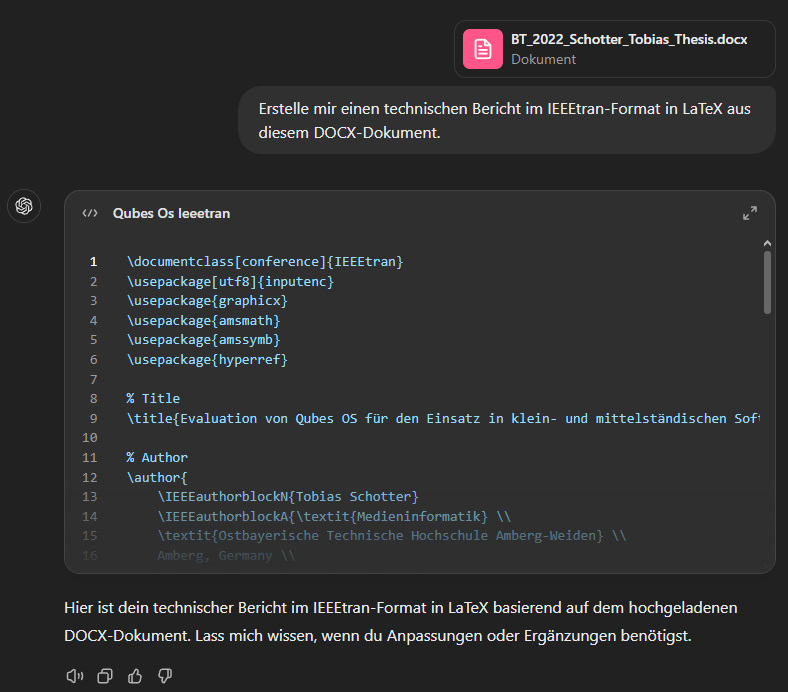
\includegraphics[width=1\linewidth]{Images/DOCXzuLaTeX.png}\\
\caption{Chat\ac{GPT} Test 2: Prompt; Testdokument \cite{schotter_tobias_2022bt}}
\label{fig:docxzulatexgpt}
\end{figure}

\begin{figure}[H]
\centering

\includegraphics[width=1\linewidth]{Images/docxzulatex.pdf}\\
\caption{Chat\ac{GPT} Test 2: Ergebnis; Testdokument \cite{schotter_tobias_2022bt}}
\label{fig:docxzulatexresult}
\end{figure}

\section{ChatGPT Test 3}

\begin{figure}[H]
\centering
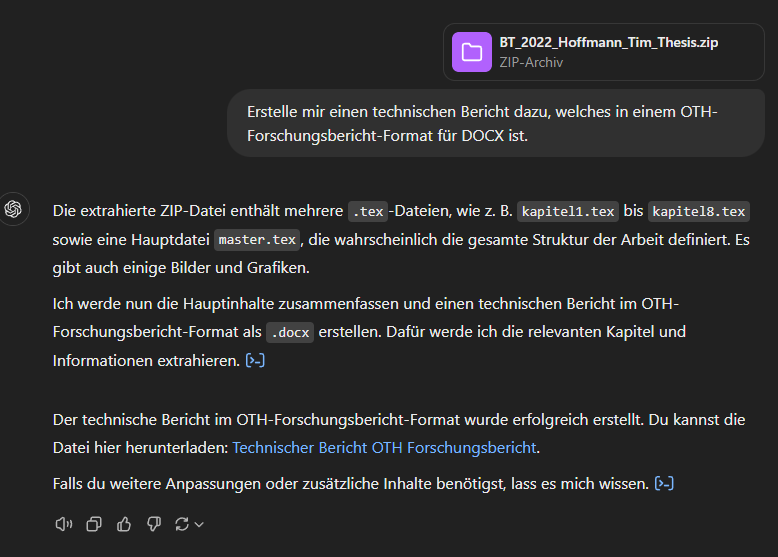
\includegraphics[width=1\linewidth]{Images/ZIPzuDOCX.png}\\
\caption{Chat\ac{GPT} Test 3: Prompt; Testdokument \cite{hoffmann_tim_2022bt}}
\label{fig:latexzudocxgpt}
\end{figure}

\begin{figure}[H]
\centering

\includegraphics[width=1\linewidth]{Images/chatgpt_oth_forschungsbericht.pdf}\\
\caption{Chat\ac{GPT} Test 3: Ergebnis; Testdokument \cite{hoffmann_tim_2022bt}}
\label{fig:latexzudocxresult}
\end{figure}

\section{ChatGPT Test 4}

\begin{figure}[H]
\centering

\includegraphics[width=1\linewidth]{Images/DOCXzuDOCX.png}\\
\caption{Chat\ac{GPT} Test 4: Prompt; Testdokument \cite{schotter_tobias_2022bt}}
\label{fig:docxzudocx}
\end{figure}


\chapter{Codeauszüge}

\section{Text-Filterungen}

\begin{listing}[H]
\begin{minted}[
frame=lines,
bgcolor=base,
fontsize=\footnotesize,
linenos
]
{typescript}
export function cleanLatexText(latexContent: string): string {
    // lösche alles vor \chapter{}
    const chapterStartIndex = latexContent.search(/\\chapter\{/);
    if (chapterStartIndex !== -1) {
      latexContent = latexContent.substring(chapterStartIndex);
    }
  
    // Regex für commands
    const commandRegex = /\\[a-zA-Z]+\{[^}]*\}|\\[a-zA-Z]+\[[^\]]*\]|\\[a-zA-Z]+/g;
    // Regex für kommentare
    const commentRegex = /%.*$/gm;
    // Regex für begin & end
    const beginRegex = /\\begin\{[^}]*\}[\s\S]*?\\end\{[^}]*\}/g;
    // Regex für whitespace
    const whitespaceRegex = /\s+/g;
    
    let filteredContent = latexContent
      // Entfernt Kommentare
      .replace(commentRegex, '')
      // Entfernt Begin/End
      .replace(beginRegex, '')
      // Entfernt Commands außer Chapter
      .replace(commandRegex, (match) => {
        return match.startsWith('\\chapter{') ? match : '';
      })
      // Entfernt whitespace
      .replace(whitespaceRegex, ' ')
      .trim();
    
    return filteredContent;
}
\end{minted}
\caption{Funktion für die LaTeX-Text-Filterung}
\label{lst:LaTeX-Text-Filterung}
\end{listing}

\begin{listing}[H]
\begin{minted}[
frame=lines,
bgcolor=base,
fontsize=\footnotesize,
linenos
]
{typescript}
export function removeSpecialChars(section: string): string {
 // entfernt '1.' '2.' etc. am anfang von einer section und special chars
 return section.replace(/\\section\{\d+\.\s*/g,'\\section{').replace(/[&#%_^~$]/g,'');
}
\end{minted}
\caption{Funktion für die SpecialChar-Filterung}
\label{lst:SpecialChar-Filterung}
\end{listing}

\section{DOCX-Dokument Generierung}

\begin{listing}[H]
\begin{minted}[
frame=lines,
bgcolor=base,
fontsize=\footnotesize,
linenos
]
{typescript}
async function PutDocxStyle(title: string, author: string, content: string) {
const doc = new Document({
sections: [
{
properties: {},
children: [
// Titel
new Paragraph({
text: title,
heading: HeadingLevel.TITLE,
alignment: AlignmentType.CENTER,
}),
// Leerzeile
new Paragraph({ text: "" }),
// Autor
new Paragraph({
alignment: AlignmentType.CENTER,
children: [
 new TextRun(author),
 new TextRun({ text: 'Fakultät Elektrotechnik, Medien und Informatik', break: 1 }),
 new TextRun({ text: 'Ostbayerische Technische Hochschule Amberg-Weiden', break: 1 }),
 new TextRun({ text: 'Amberg, Deutschland', break: 1 }),
 ],
}),
// Leerzeile
new Paragraph({ text: "" }),
// Content
...content.split('\n').map((sectionText) => {
 if (sectionText.startsWith('\\section')) {
    return new Paragraph({
     text: sectionText.replace('\\section', '').replace(/[{}]/g, ''),
     heading: HeadingLevel.HEADING_1,
    });
 } else {
    return new Paragraph({
     text: sectionText,
    });
 }
}),
],
},
],
});

 const buffer = await Packer.toBuffer(doc);
 return buffer;
}
\end{minted}
\caption{Generierung eines \ac{DOCX}-Dokuments für die Ausgabe}
\label{lst:docx-gen}
\end{listing}